\chapter{Grundlagen}
Zu den Grundlagen dieser Arbeit zählen Theorien und Konzepte aus dem Geomarketing und der Geoinformatik sowie die angewendeten Technologien im Prototyp.
Die folgenden Kapitel stellen die wichtigsten Informationen bereit, die ein allgemeines Verständnis der Anwendung ermöglichen.

\section{Geomarketing}
Aus dem Handbuch Geomarketing von Michael Herter: 
Geomarketing analysiert aktuelle wie potenzielle Märkte nach räumlichen Strukturen, um den Absatz von Produkten effektiver planen und messbar steuern zu können \footcite{herter_handbuch_2018}.
Ergänzend befasst sich Geomarketing mit der Beschreibung, Analyse und dem Vergleich beliebiger Märkte und Standorte hinsichtlich ökonomischer Charakteristiken und Potenziale durch Referenzierung und flächendeckende Berechnung von Marktdaten auf geographische Strukturen \footcite{geomarketing_def}.
Kurz gesagt beschreibt Geomarketing also sämtliche Aspekte des Marketings, die einen geografischen Bezug haben.

Zu relevanten Themenbereichen des Geomarketings für diese Arbeit gehören Standortanalyse /-planung, Filialplanung sowie die Gravitationsanalyse und das Konzept des Gravitationsmodels.
Weiterhin werden die Begriffe Geodaten und Marktdaten erläutert.

\subsection{Standortanalyse}
Allgemein erörtert die Standortanalyse Beschreibung, Untersuchung und Unterscheidung von guten und schlechten IST-Standorten sowie potenziellen neuen Standorten und deren Umfeld hinsichtlich der Eignung für den Absatz bestimmter Produkte \footcite{geomarketing_standortanalyse}.

Für die Betrachtung von potenziellen neuen Standorten werden unternehmensinterne Daten (falls vorhanden) und externe Daten anhand von verschiedenen Standortfaktoren untersucht, mit dem Ziel sämtliche potenzielle Standorte auf möglichst wenig Alternativen zu begrenzen und schließlich analytisch die beste zu bestimmen. 
Die Unterscheidung kann hierbei in höchster Ebene in vier Kategorien erfolgen \footcite{haas_standortfaktoren}:

\textbf{\emph{Zugehörigkeit zur Leistungserstellung}} beinhaltet Faktoren zur Beschaffung, Produktion und zum Absatz.

\textbf{\emph{Grad der monetären Quantifizierbarkeit}} beinhaltet harte und weiche Standortfaktoren. 
Harte Standortfaktoren sind immer quantifizierbar und dienen daher als Grundlage für wirtschaftliche Berechnungen und Kosten.
Der Einfluss weicher Standortfaktoren kann nicht eindeutig bestimmt werden und kann mit der selektiven Clusterung all der Faktoren beschrieben werden, die auf dem individuellen Raumempfinden der Menschen in ihrer Lebens- und Arbeitswelt basieren.

\textbf{\emph{Maßstabsebene}} beschreibt Faktoren der Makro-, Meso- und Mikroebene oder anders der Länder-, Region- und Gemeindeebene.

\textbf{\emph{Grad der Spezifität}} beschreibt Sektor- und Branchenspezifische Faktoren.

Die Abbildung \ref{img:standortfaktoren} bietet hierzu eine detaillierte Auflistung der Kategorien mit Beispielen.

\begin{figure}[H]
	\centering
	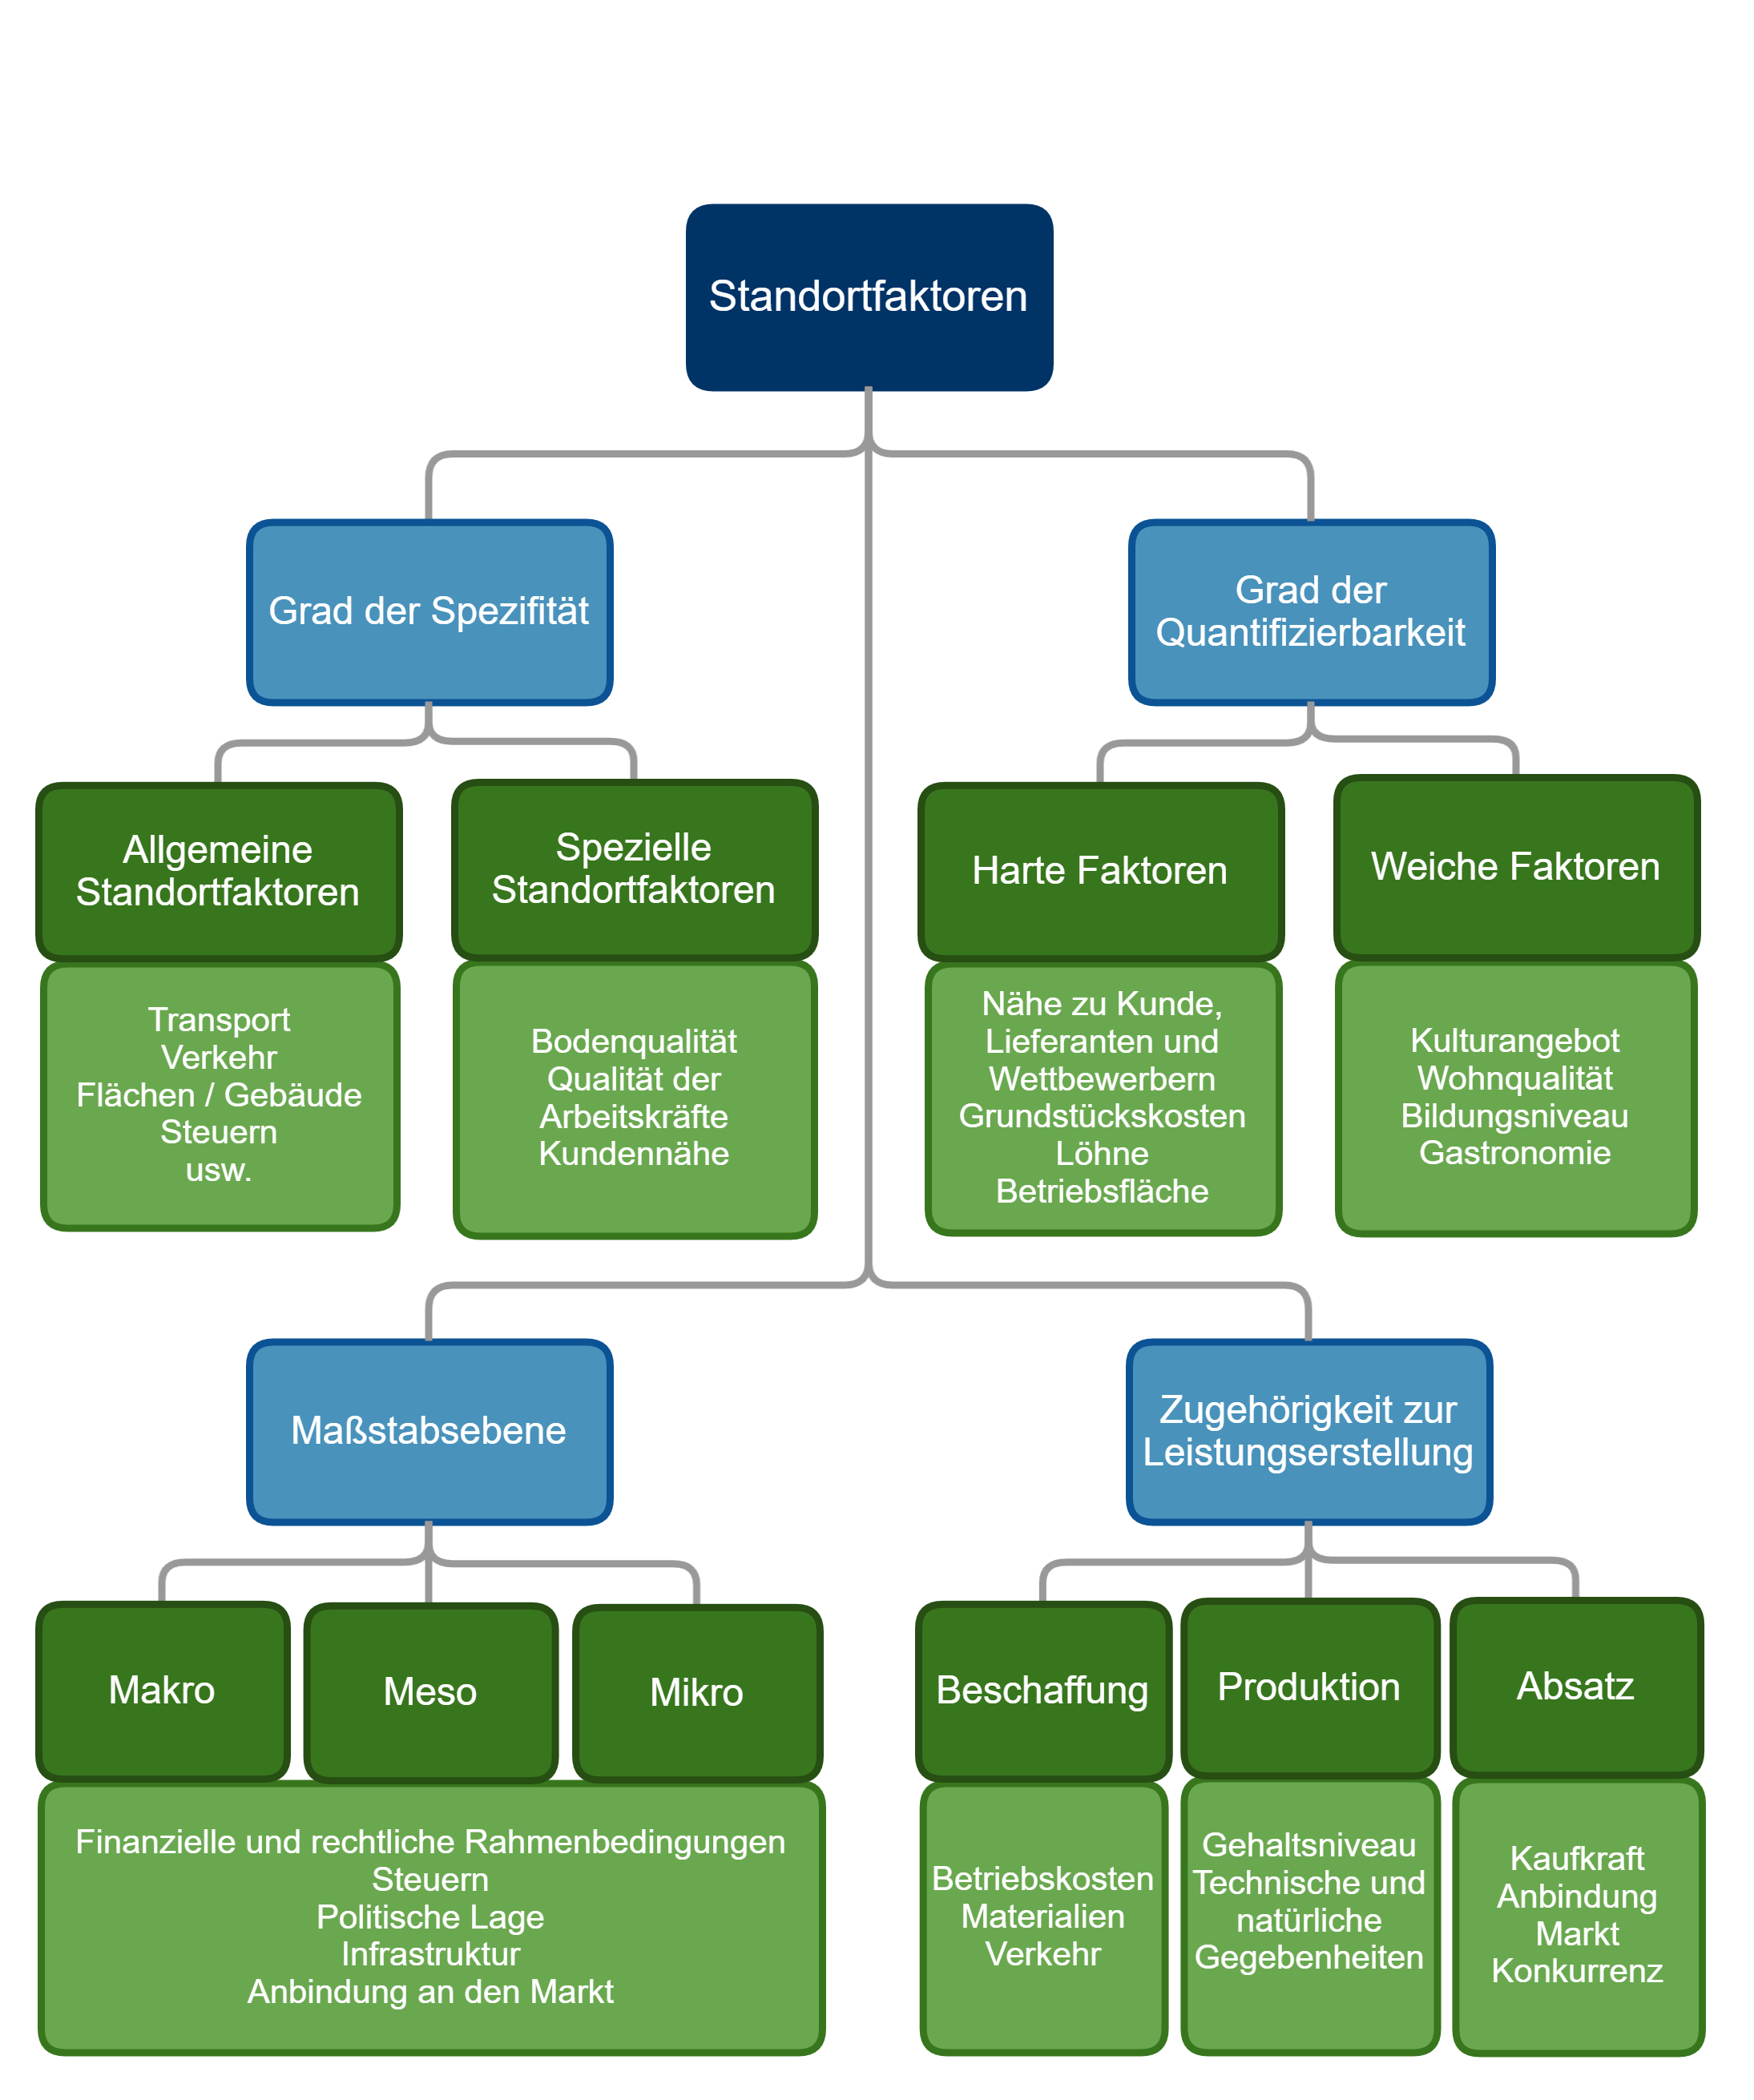
\includegraphics[scale=0.2]{resources/images/Standortfaktoren.png}
	\caption{Eigene Darstellung Standortfaktoren}
	\title{Standortfaktoren}
	\label{img:standortfaktoren}
\end{figure}

\newpage
Weitere zusätzlich relevante Aspekte können sein:
\begin{itemize}
	\item Zielgruppe: Wer sind die Kunden? Ist das Verkaufsmodell B2C oder B2B?
	\item Demografische Merkmale: Alter, Geschlecht und Wohnort der Kunden
	\item Sozioökonomische Betrachtung: Gibt es einen Zusammenhang zwischen Beruf, Bildungsstand oder Einkommen und dem Kaufverhalten?
	\item Psychografische Merkmale: Haben der Lebensstil, Werte, Motivation oder Ähnliches Einfluss auf das Kaufverhalten?
	\item Wettbewerbsdichte
	\item Preispolitik der Wettbewerber
	\item Größe des Einzugsgebiets
	\item Kaufkraftwerte des Gebiets
	\item Erreichbarkeit
	\item Mietpreise
	\item Attraktivität des Standortes
\end{itemize}

Obwohl Filialen geographisch aus betriebswirtschaftlicher Sicht Unternehmensstandorte sind, kann zwischen Filialplanung und Standortplanung unterschieden werden und dementsprechend werden andere Faktoren bei der Standortanalyse wichtiger oder hinzugezogen.
Für die Filialplanung zusätzlich relevant werden folgende Faktoren:

\begin{itemize}
	\item Bekanntheitsgrad, Markenstärke: Was zeichnet die eigene Marke aus? Was setzt sie ab?
	\item Freies Potential: Herrscht genug Nachfrage?
	\item Kannibalisierungs-Effekte: Ist der Standort zu nah an anderen, bestehenden Filialen?
	\item Logistikkosten: Kann ich Lieferwege und Lagerstandorte optimal nutzen?
\end{itemize}

Für eine einfache mathematische Standortanalyse können nun zunächst die Kategorien anhand der eigenen Marke als mehr oder weniger relevant bewertet und gewichtet werden.
Außerdem müssen die einzelnen Kategorien für jeden Standort bewertet werden. 
Die Bewertungen der Kategorien müssen nun mit der Gewichtung der Kategorie multipliziert werden, um die genaue Faktorbewertung des Standorts für jede Kategorie zu erhalten. 
Die Faktorbewertungen summiert ergeben nun Standortbewertung. 
Sind die Standortbewertungen tabellarisch aufgelistet und werden anschließend verglichen ist die Standortanalyse abgeschlossen.

\subsection{Standortplanung/ Filialplanung}
Bereits im vorherigen Kapitel erwähnt, wird zwischen der Standortplanung und der Filialplanung geringfügig unterschieden.
So legt die Filialplanung ihren Fokus auf mehrere in einem Filialnetz zusammengefasste Standorte, welche bei der Analyse berücksichtigt werden müssen.
Die Standortplanung konzentriert sich dagegen eher auf einzelne Standorte.

Beide Methoden verwenden jedoch in der vorher durchgeführten Standortanalyse herausgestellte Erkenntnisse, um die potenziellen Standorte einzuordnen und eine Entscheidung für die nächste Filialeröffnung zu treffen.

\subsection{Geodaten}
Geodaten sind strukturierte codierte Angaben zur quantitativen und qualitativen Beschreibung von natürlichen oder definierten Objekten der realen Welt. 
Geodaten vermessen die Welt und beschreiben geographische (Teil-)räume und Orte \footcite{geomarketing_geodaten}.

Geodaten werden in mehrere Typen klassifiziert und unterliegen definierten Standards, die sich am Markt durchgesetzt haben \footcite{gistandards.eu}.

So definiert die ISO 19115 einen Standard zur Beschreibung geographischer Informationen anhand von Metadaten \footcite{19115_iso}.
Wichtigste standardisierte Dienste sind unter anderem:

\begin{itemize}
	\item WMS: Web Map Service zum Teilen von Karten
	\item WFS: Web Feature Service zum Teilen von Feature-Daten
\end{itemize}

Zu den wichtigsten standardisierten Datenformaten zählen:

\begin{itemize}
	\item GeoJSON - JSON Format mit Geo-Spezifika
	\item KML - Keyhole Markup Language 
	\item GPKG - GeoPackage definiert vom Open Geospatial Consortium
\end{itemize}

Im Prototyp verwendete Formate sind GeoJSON für Features sowie einfache Bilder (PNG) der Hintergrundkarte.

\subsection{Marktdaten}
Marktdaten oder Marktinformationen beschreiben die individuelle regionale Charakteristik geographischer Gebiete oder Standorte mittels qualitativer Merkmale \footcite{geomarketing_marktdaten}.

Es gibt unternehmensinterne sowie externe Marktdaten.
Marktdaten können aus einem internen CRM-System stammen und über Umfragen, Marktforschung und Erhebungen als Primärdaten selbst erhoben werden oder aus staatlichen Statistiken sowie Branchen- und Wirtschaftsverbänden als Sekundärdaten eingeholt werden.

Im Prototyp verwendete Marktdaten sind aus Sekundärdaten erstellte Beispieldaten für Filialen und Gebiete.

\section{Geoinformationssysteme}
\label{sec:gis}
Geoinformationssysteme, kurz GIS, sind Informationssysteme zur Erfassung, Bearbeitung, Organisation, Analyse und Präsentation räumlicher Daten \footcite{geomarketing_gis}.  
Ähnlich anderer Informationssysteme besteht ein GIS aus Hardware (Computer, Server, Drucker etc.), Software mit Analyse-Tools (Zeichnen, Kalkulation) und räumlichen Daten (Koordinatensystem, Karten, Geometrien etc.). 
Gegebenenfalls wird die Liste um eine Verwaltungsebene ergänzt sobald ein Berechtigungskonzept für die Daten und Funktionen des GIS angewendet wird.
Erste GIS Systeme stammen aus den sechziger Jahren (Canada Geographic Information System \footcite{esri_cgis}). 
Zu den ersten Nutzern der Systeme gehörten vor allem Behörden und Universitäten, so wurden viele grundlegende theoretische Konzepte an der Harvard University von Professor Howard Fisher aufgestellt \footcite{gis_harvard_2005}.
Mittlerweile haben sich viele Web-GIS etabliert, hierbei wird das Informationssystem über eine Website veröffentlicht oder benutzt. 
Zu den größten Vertretern moderner Web-GIS zählen vor allem Google Maps, Bing Maps, OpenStreetMaps als OpenSource-Alternative oder etwas kleinere Anbieter wie HERE oder Yandex.Maps.
Kommerzielle Web-GIS bieten meist ein eingeschränktes Funktions-Set, was sie nicht als Produkt für individuelle Software-Lösungen für Firmen in Frage kommen lässt. Daher greifen viele Firmen auf kommerzielle Desktop-GIS zurück oder lassen sich ganz individuelle Systeme bauen, die aus Web- und Desktop-GIS bestehen.
Zu den bekanntesten GIS zählen Produkte von ESRI, Autodesk, Pitney Bowes oder CAIGOS. 

In der Geophysik wird die Erde nicht als Kugel, sondern als Ellipsoid bezeichnet \footcite{jung_figur_1956}.
Wenn man jedoch eine Karte elektronisch auf einem Bildschirm betrachtet, dann sieht man ein Rechteck und keine Anzeichen der Krümmung eines Globus.
Die Problematik der Projektion der Erde auf eine flache Darstellung hat über den Lauf der Jahre mehrere Lösungen produziert, die jedoch alle mit Koordinatensystemen und Projektionsrechnungen zu tun haben und bietet Stoff für ein eigenes Wissenschaftsfeld.
Aufgrund dessen versuchen die nächsten Zeilen, die Problematik und Anwendung im Prototyp kurz zu beschreiben.

In einem GIS muss die Projektion zwangsläufig enthalten sein und das bestenfalls für mehrere Projektionstypen.
Die meisten Web-Karten wie Google Maps oder Bing Maps benutzen die Projektion World Geodetic System 1984 (kurz WGS 84) mit dem Koordinatenreferenzsystem (engl. CRS) der European Petroleum Survey Group (kurz EPSG) 4326, welches Koordinaten in Grad darstellt \footcite{epsg.io_4326}.
OpenLayers hingegen benutzt standardmäßig WGS 84 mit EPSG 3857, welches Koordinaten in Metern zur Ursprungskoordinate darstellt \footcite{epsg.io_3857}.
Die Abbildung \ref{img:epsg.io} zeigt die Koordinaten eines Punktes in Berlin in beiden Koordinatenreferenzsystemen.

\begin{figure}[H]
	\centering
	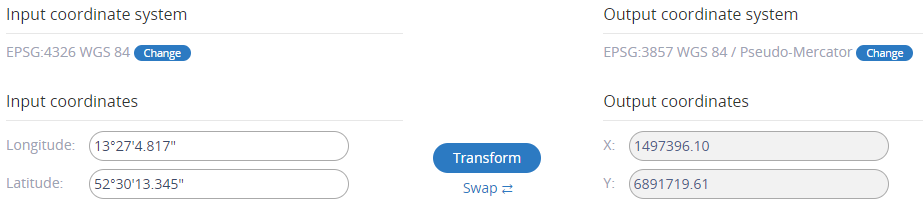
\includegraphics[scale=0.6]{resources/images/projection_epsg.png}
	\caption{Bildschirmaufnahme der Transformation  von EPSG 4326 zu EPSG 3857 von epsg.io \footcite{epsg.io_transform}}
	\label{img:epsg.io}
\end{figure}

Im Wesentlichen werden im Prototyp die oben beschriebenen Projektionen verwendet.
Die Geodaten der Filialen sowie der Zensusgebiete sind in EPSG 4326 erfasst und müssen dementsprechend vor der Darstellung transformiert werden.
Entsprechende Funktionen sind im Kapitel \ref{ch:implementierung} \glqqImplementierung\glqq beschrieben.

\section{Genutzte Technologie}
Für die prototypische Ausarbeitung des Modells wurde auf modernste Technologien und Frameworks zugegriffen. So wird als Karten-Framework /gls(ol) in der Version 6.4.3 verwendet sowie /gls(angular) in der Version 10.
Die Darstellung \ref{img:tech_stack} zeigt die genutzten Technologien als Grafik.

\begin{figure}[H]
	\centering
	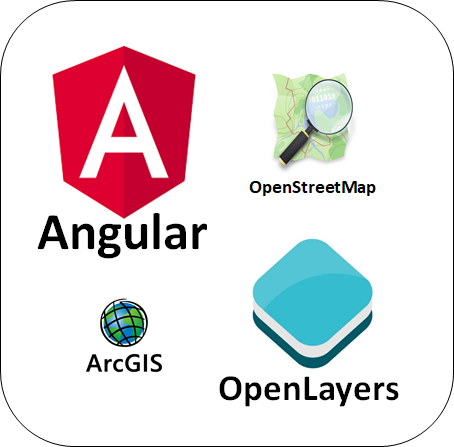
\includegraphics[]{resources/images/tech_stack.png}
	\caption{Eigene Abbildung des Technologie Stacks der Anwendung}
	\label{img:tech_stack}
\end{figure}

OpenLayers bietet ein breites Portfolio an Funktionen und Features passend für sämtliche Anforderungen realer Geo-Informationssysteme, die in der Praxis verwendet werden. 
Im Bezug auf die prototypische Anwendung dieser Arbeit sind vor allem die Unterstützung der Darstellung von Punkten (Filialen) und der Zensusgebiete in GeoJSON-Format auf verschiedenen Layern notwendig sowie die einfache Konfigurierbarkeit von Karten-Interaktionen, wie zum Beispiel das Platzieren, Verschieben und Editieren von Punkt-Objekten (Filialen) auf der Karte.

Weiterführend soll die Anwendung schnell, kompakt und modern sein, um die Relevanz aus Gründen der Performance auf dem Markt gewährleisten zu können. 
Daher erfolgt die Umsetzung mit dem auf TypeScript basierenden Framework Angular. Besonderes Augenmerk liegt hierbei im Prototyp eigentlich nur auf der simplen, kompakten und schnellen Auslieferung eines Web-Servers als Host der Anwendung. Zu den für die weiterführende Entwicklung relevant werdenden Features des Frameworks zählen eine große Community, einen fortlaufenden Support sowie eine fortlaufende Entwicklung durch Google, die Verwendung von TypeScript, einem Superset von JavaScript mit verbesserter Funktionalität und sämtlichen Features, die für Entwicklung einer effizienten und anspruchsvollen Single-Page-Webanwendung benötigt werden. 